\section{Обзор существующих решений}
\label{sec:Section2} \index{Section2}

\subsection{Микроархитектура процессора}

    Современный CPU (Central Processing Unit -- центральный процессор) представляет собой
    систему взаимосвязанных между собой процессорных ядер, не обязательно одинаковых.

    Исполнение инструкции современным процессорным ядром является многостадийным pipeline'ом
    (конвейером) из различных блоков. В зависимости от исполняемого workload'а утилизируются
    различные блоки, поэтому скорость исполнения workload'а сильно зависит от его особенностей
    (типа).

    В наиболее общем виде можно разбить pipeline исполнения инструкции на процессоре на несколько
    последовательных стадий:
    \begin{enumerate}
        \item Fetching (чтение инструкции из памяти);
        \item Decoding (декодирование прочитанной инструкции);
        \item Execution (исполнение инструкции);
        \item Memory (чтение/запись в память при необходимости);
        \item Writeback (запись результата инструкции в регистры процессора).
    \end{enumerate}

    Чаще всего приведённые выше стадии дробятся на более локальные стадии, применяются
    дополнительные оптимизации для ускорения исполнения инструкций а также их распараллеливания
    (например, кеширование декодированных инструкций и предсказатель ветвлений). Наиболее
    актуальным примером являются OoO (Out-of-Order -- внеочередное исполнение) процессоры,
    в которых используется алгоритм Томасуло, позволяющий реализовать
    исполнение машинных инструкций не в порядке их следования в машинном коде, а в порядке
    готовности к выполнению, за счёт чего значительно увеличивается скорость исполнения инструкций.

    В типичной реализации OoO используется ROB (Re-order buffer), который представляет собой
    циклический буфер и накапливает инструкции для обеспечения возможности их переупорядочить.
    Обычно в ROB попадают не исходные машинные иструкции, а прошедшие через стадию register-renaming
    (переименование регистров) для избавления от data-hazards (зависимости по данным), а значит для
    дополнительного распараллеливания инструкций.

    Наибольший интерес в данной работе представляет организация обращения процессора в память,
    также затрагивается аспекты, связанные с OoO исполнением.

    \begin{figure}[!h]
        \caption{Схема конвейера процессора Arm Cortex A77 \cite{CortexA77Docs}}
        \centering
        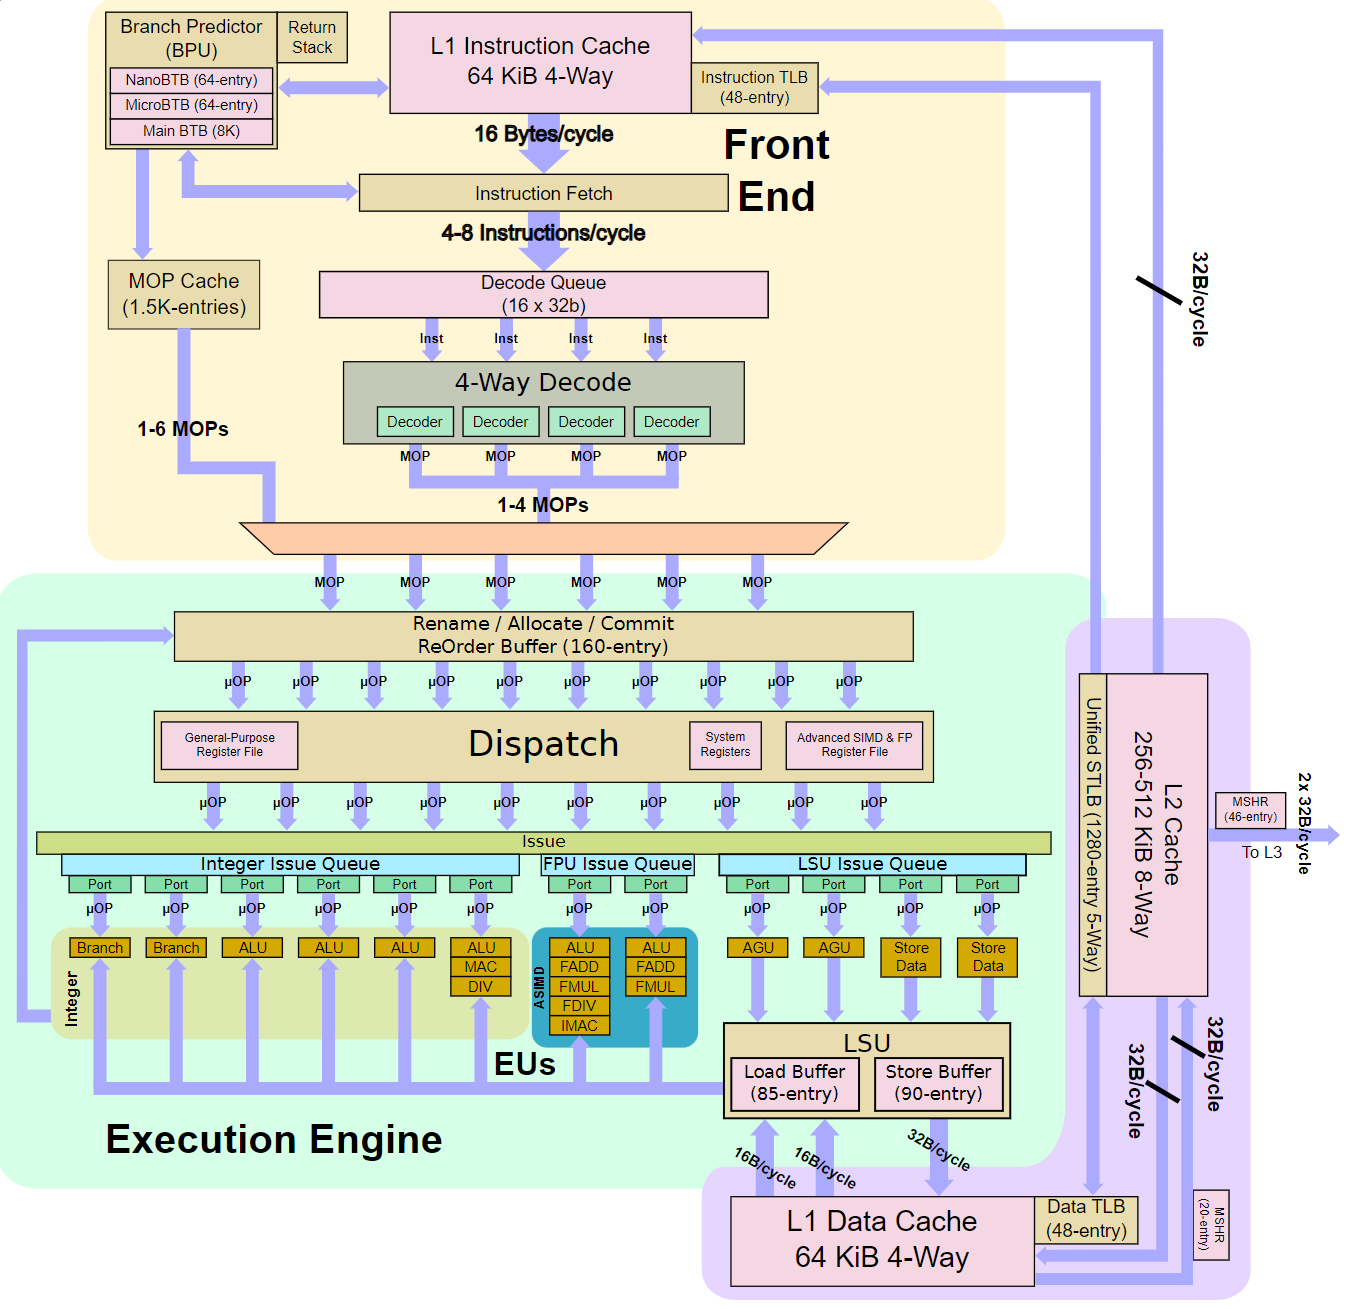
\includegraphics[width=161mm]{CortexA77}
        \label{cortexA77}
    \end{figure}

\subsection{Подсистема памяти в современных SoC}

    Процессор в современным мобильных системах встроен в так называемую SoC (System-on-chip --
    система на кристалле) систему -- электронная схема, которая выполняет цели компьютера
    и размещена на одной интегральной схеме. Таким образом, в такую систему встроены сразу CPU,
    таймеры, счётчики, интерфейсы для периферийных устройств, ОЗУ, ПЗУ и даже GPU
    (Graphics Processing Unit -- графический процессор). Именно таким образом устроены современные
    смартфоны, фотоаппараты, умные часы, элекронные книги и схожие устройства.

    Одна из подсистем SoC,

\subsection{Исследования на тему bandwidth и latency}

    [TODO] В работе \cite{clapp2015quantifying} рассматривается подход использования аналитической
    формулы влияния bandwidth и latency памяти на производительность суперскалярного
    процессора в рамках рабочих нагрузок, связанных с big data областью. В этом подходе
    используется схожий принцип, предлагаемых в данной работе: использование показателя
    $cpi$, который включает в себя слагаемые, связанные с циклами, потраченными на время
    ожидания транзакций-обращений в память. Авторы исследуют влияние значений bandwidth
    и latency на производительность, которую они выражают через $cpi$, для различных workload'ов:
    latency-bound и bandwidth-bound. Однако данное исследование ограничивается
    рассмотрением обращений только в DDR память при фиксированных частотах всех устройств.

    [TODO] Авторы работы \cite{keramidas2010interval} предлагают 2 модели для учёта latency памяти
    в рамках DVFS алгоритма. Первая модель разбивает циклы CPU на 2 компоненты: относящиеся
    к ожиданию транзакций памяти и относящиеся непосредственно к вычислительным блокам CPU.
    Утверждается, что при изменении частоты CPU изменяются только циклы, относящиеся к памяти,
    на этом и основывается алгоритм DVFS, использующий перерасчёт времени исполнения через
    циклы при различных частотах CPU. Вторая модель является модификацией-улучшением первой модели:
    дополнительно предполагается, что в группе инструкций, которые обращаются в память подряд,
    следует учитывать только первую инструкцию в формуле для перерасчёта циклов, которые относятся
    к памяти, однако это требует наличие дополнительной информации на уровне кешей: среди всех
    промахов в кеши (т.е. обращений в следующий уровень памяти) следует учитывать только первые
    промахи среди группы промахов (промахов, находящихся на расстоянии порядка latency обращения
    в вышележащие уровни памяти во времени).

    В работе также отмечается, что следует учитывать ROB в OoO процессорах: из циклов, относящихся к
    транзакциям памяти, следует вычесть ту часть циклов, которую тратит CPU на исполнение
    инструкций, расположенных в логическом порядке после инструкции-обращений в память,
    так как такие инструкции исполняются спекулятивно.



\subsection{Симулятор архитектуры Gem5}

\subsection{Capacity Awate Scheduling в ядре Linux}

\subsection{DVFS алгоритмы}


%%About PMU counters (from arm site)
%%About Gem5 PMU implementation

\newpage
